% Name: Instruction pipeline
% Description: Five instructions moving through the five classic stages, one cycle apart.
% Tags: pipeline, CPU, computer architecture, RISC

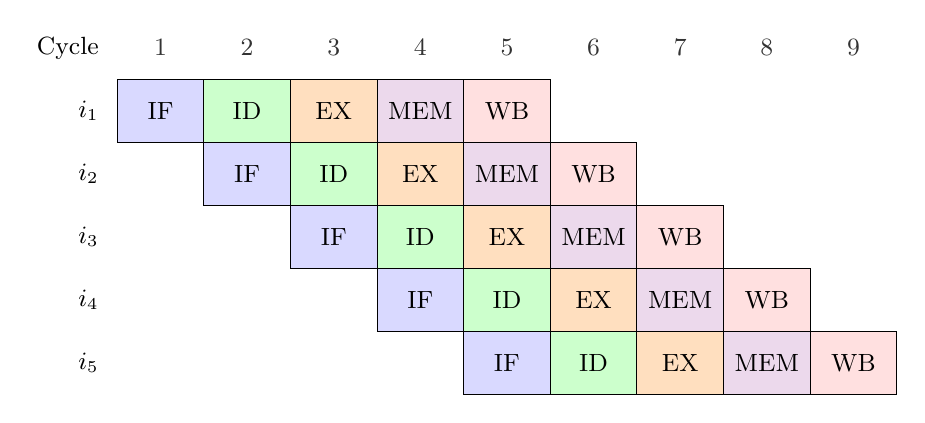
\begin{tikzpicture}[x=11mm, y=8mm, every node/.style={font=\small}]
  \node[anchor=east] at (0.4,1) {Cycle};
  \foreach \c in {1,...,9}
    \node[gray!40!black] at (\c,1) {\c};
  \foreach \i in {1,...,5} {
    \node[anchor=east] at (0.4,1-\i) {$i_{\i}$};
    \foreach \s/\stage/\col in {0/IF/blue!15, 1/ID/green!20, 2/EX/orange!25, 3/MEM/violet!15, 4/WB/red!12}
      \node[draw, fill=\col, minimum width=11mm, minimum height=8mm] at (\i+\s,1-\i) {\stage};
  }
\end{tikzpicture}
